{\fontsize{12pt}{22pt} \textbf{ROC curve}\par}

\vspace{5mm}

ROC = Receiver Operating Curve

ROC curve is used essentially for binary classification.

\vspace{5mm}

\underline{Use of the ROC curve}

\vspace{5mm}

One model:

We use ROC curve to evaluate the performance of one classifying model that we can obtain when varying a threshold.

\vspace{5mm}

Several models:

We use ROC curve to compare several classifying models in evaluating the area under the curve (AUC) for a range of threshold.

\vspace{5mm}

\underline{Intuition}

\vspace{5mm}

After running the prediction of a specific model, we draw the confusion matrix (actual vs predited) with a certain threshold.

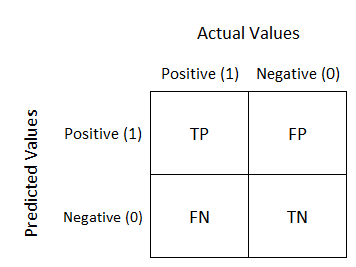
\includegraphics[scale=0.5]{../images/confusionmatrice.png}

\vspace{5mm}

We then modify the threshold and draw another confusion matrix.

The ROC graph summarizes all of the confusion matrices that each threshold produced.

\vspace{5mm}

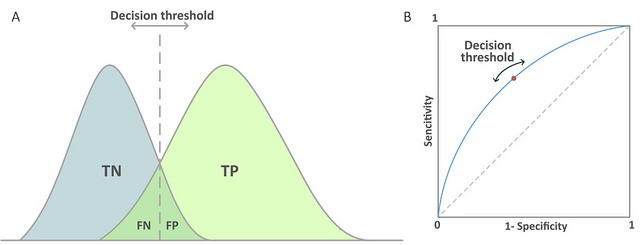
\includegraphics[scale=0.5]{../images/overlap_roc.jpeg}

\vspace{5mm}

On the left picture we see the ability of a model to give a clear distinction between the two classes. The curves are drawn from the predictions and the actual results)

\vspace{5mm}

\underline{Implementation}

\vspace{5mm}

1. Get probability predictions

2. Sort the probabilities (prediction)

3. Sort the validation (actual) according to previous sort

4. Loop on the sorted validation. At each iteration:

- increment TP or FP

- compute the TPR and FPR.

5. Plot (FPR, TPR)

\vspace{5mm}

See \textit{https://docs.eyesopen.com/toolkits/cookbook/python/plotting/roc.html} for an implementation example, or data challenge Face\_Recognition.

\vspace{5mm}
